\documentclass[xcolor=table]{beamer}\usepackage[]{graphicx}\usepackage[]{color}
% maxwidth is the original width if it is less than linewidth
% otherwise use linewidth (to make sure the graphics do not exceed the margin)
\makeatletter
\def\maxwidth{ %
  \ifdim\Gin@nat@width>\linewidth
    \linewidth
  \else
    \Gin@nat@width
  \fi
}
\makeatother

\definecolor{fgcolor}{rgb}{0, 0, 0}
\newcommand{\hlnum}[1]{\textcolor[rgb]{0.502,0,0.502}{\textbf{#1}}}%
\newcommand{\hlstr}[1]{\textcolor[rgb]{0.651,0.522,0}{#1}}%
\newcommand{\hlcom}[1]{\textcolor[rgb]{1,0.502,0}{#1}}%
\newcommand{\hlopt}[1]{\textcolor[rgb]{1,0,0.502}{\textbf{#1}}}%
\newcommand{\hlstd}[1]{\textcolor[rgb]{0,0,0}{#1}}%
\newcommand{\hlkwa}[1]{\textcolor[rgb]{0.733,0.475,0.467}{\textbf{#1}}}%
\newcommand{\hlkwb}[1]{\textcolor[rgb]{0.502,0.502,0.753}{\textbf{#1}}}%
\newcommand{\hlkwc}[1]{\textcolor[rgb]{0,0.502,0.753}{#1}}%
\newcommand{\hlkwd}[1]{\textcolor[rgb]{0,0.267,0.4}{#1}}%
\let\hlipl\hlkwb

\usepackage{framed}
\makeatletter
\newenvironment{kframe}{%
 \def\at@end@of@kframe{}%
 \ifinner\ifhmode%
  \def\at@end@of@kframe{\end{minipage}}%
  \begin{minipage}{\columnwidth}%
 \fi\fi%
 \def\FrameCommand##1{\hskip\@totalleftmargin \hskip-\fboxsep
 \colorbox{shadecolor}{##1}\hskip-\fboxsep
     % There is no \\@totalrightmargin, so:
     \hskip-\linewidth \hskip-\@totalleftmargin \hskip\columnwidth}%
 \MakeFramed {\advance\hsize-\width
   \@totalleftmargin\z@ \linewidth\hsize
   \@setminipage}}%
 {\par\unskip\endMakeFramed%
 \at@end@of@kframe}
\makeatother

\definecolor{shadecolor}{rgb}{.97, .97, .97}
\definecolor{messagecolor}{rgb}{0, 0, 0}
\definecolor{warningcolor}{rgb}{1, 0, 1}
\definecolor{errorcolor}{rgb}{1, 0, 0}
\newenvironment{knitrout}{}{} % an empty environment to be redefined in TeX

\usepackage{alltt}

\usepackage[]{graphicx}\usepackage[]{color}

\usepackage{alltt}
\usepackage{hyperref}

\usepackage{array}
\usepackage[originalparameters]{ragged2e} 

% kable packages
\usepackage{longtable}
\usepackage{array}
\usepackage{multirow}
\usepackage{wrapfig}
\usepackage{float}
\usepackage{colortbl}
\usepackage{pdflscape}
\usepackage{tabu}
\usepackage{threeparttable}
\usepackage{threeparttablex}
\usepackage[normalem]{ulem}
\usepackage{makecell}

\usepackage{amsmath}
\usepackage{booktabs}
%\usepackage[ansinew]{inputenc}
\usepackage[utf8]{inputenc}
\usepackage[ngerman, english]{babel}

\usepackage{bm}

\usetheme{metropolis}   



\IfFileExists{upquote.sty}{\usepackage{upquote}}{}
\begin{document}

\title{Programming with R/Advanced R}
\institute{FDZ Spring Academy}


\author[Dries Debeer \& Benjamin Becker]{Dries Debeer \& Benjamin Becker}
\date{18. and 19. March 2021}


\begin{frame}
\titlepage
\end{frame}
\addtocounter{framenumber}{-1}

\begin{frame}{Introduction}
\textbf{Who are we?}

\begin{columns}[t]
\begin{column}{.475\textwidth}
\textcolor{mLightBrown}{Dries Debeer}
\end{column}
  \begin{column}{.475\textwidth}
    \textcolor{mLightBrown}{Benjamin Becker}
  \end{column}
\end{columns}

\begin{columns}[t]
\begin{column}{.475\textwidth}
Researcher at KU Leuven
  	
\end{column}
\begin{column}{.475\textwidth}
Researcher at IQB (Statistics Department)

  \end{column}
\end{columns}

\vspace{0.5cm}

\begin{columns}[t]
\begin{column}{.475\textwidth}
\href{https://github.com/ddebeer/scDIFtest}{scDIFtest}, \href{https://github.com/ddebeer/permimp}{permimp}, \href{https://github.com/beckerbenj/eatATA}{eatATA}
  	
\end{column}
\begin{column}{.475\textwidth}
\href{https://github.com/beckerbenj/eatGADS}{eatGADS}, \href{https://github.com/beckerbenj/eatDB}{eatDB}, \href{https://github.com/beckerbenj/eatATA}{eatATA}, \href{https://github.com/beckerbenj/pisaRT}{pisaRT}

  \end{column}
\end{columns}

\vspace{0.5cm}

\begin{columns}[t]
\begin{column}{.475\textwidth}

\href{mailto:dries.debeer@kuleuven.be}{dries.debeer@kuleuven.be}
  	
\end{column}
  \begin{column}{.475\textwidth}

\href{b.becker@iqb.hu-berlin.de}{b.becker@iqb.hu-berlin.de}

  \end{column}
\end{columns}

\vspace{1.5em}
\end{frame}

\begin{frame}{Introduction}
\textbf{Who are you?}
\begin{enumerate}%\itemsep0em
	\item Specific interests/motivation for this workshop?
	\item Previous knowledge and experience?
	\begin{itemize}
	  \item with R
	  \item with other statistic software
	  \item with other programming languages
	\end{itemize}
\end{enumerate}
\end{frame}

\begin{frame}{Motivation}
	\begin{itemize}
			\item Being more efficient in your research
			\begin{itemize}
			  \item Save time and nerves
			  \item Avoid errors and bugs
			  \item High transfer effect to all projects (which use data)
			\end{itemize}
			\item Successful collaborations (with your future self?)
			\item Syntaxes as part of paper submissions
	\end{itemize}
\end{frame}

\begin{frame}{Motivation}
	Two of your worst enemies
	\begin{itemize}
			\item Past Self
			\begin{itemize}
			  \item Is the biggest messy in existance
			  \item Did not document anything
			  \item Uses a completely different style of writing code than yourself
			\end{itemize}
			\item Future Self
			\begin{itemize}
			  \item Has the memory of a goldfish
			  \item Will have zero understanding for your current brilliance
			\end{itemize}
	\end{itemize}
\end{frame}

\begin{frame}{Motivation}
\begin{center}
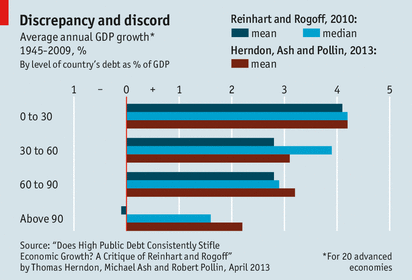
\includegraphics[width=.75\textwidth]{reinhart_rogoff.PNG}
\end{center}
\end{frame}


\begin{frame}{Motivation}
\begin{center}
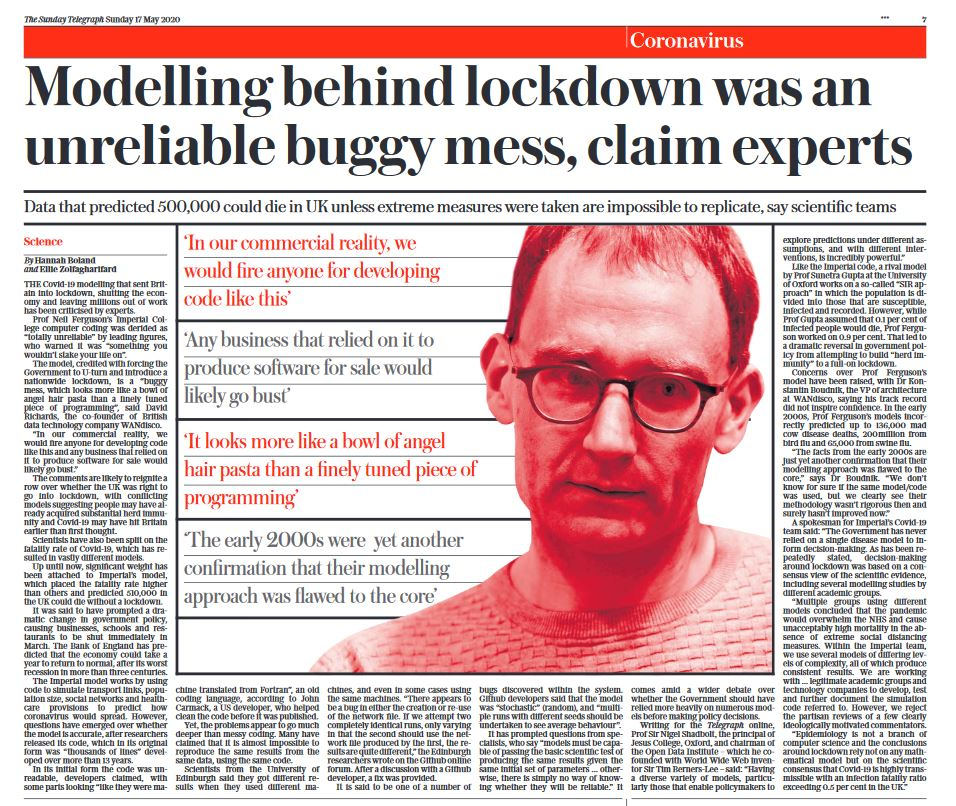
\includegraphics[width=.75\textwidth]{bad_code_media.JPG}
\end{center}
\end{frame}

\begin{frame}{Motivation}
Concept of Technical Debt
\begin{itemize}
  \item We write (messy) code for data cleaning/analyses
  \item We decide on data sets/models/graphs/tables/...
  \item We try to publish it, get a major revision
  \item We need to rerun some analyses
  \item Modifying/extending our code is more difficult than it should be
\end{itemize}
Solutions
\begin{itemize}
  \item Refactor/rewrite your could before submitting
  \item \textbf{Write better R code}
\end{itemize}
\end{frame}

\begin{frame}{Goals of this workshop}
\begin{itemize}
  \item Better practical R skills
  \item Better theoretical understanding of R (and programming)
  \item Different framing: R as a programming language
\end{itemize}
\end{frame}


\section{R Objects (Recap)}

\section{Clean Code}

\section{Iteration}

\section{Functions I}
\begin{frame}{Why?}
\begin{itemize}
  \item Readability
  \begin{itemize}
    \item Shorter
    \item Easier understanding
    \item Removes distractions, like references in a paper
  \end{itemize}
  \item Transferability
  \begin{itemize}
    \item Other use cases
    \item Other projects
    \item Other persons
  \end{itemize}
\end{itemize}
\end{frame}


\begin{frame}[fragile]{Why?}
\begin{kframe}
\begin{alltt}
\hlkwd{mean}\hlstd{(mtcars}\hlopt{$}\hlstd{mpg)}
\end{alltt}
\end{kframe}[1] 20.09062
\begin{kframe}\begin{alltt}
\hlcom{# vs.}
\hlkwd{sum}\hlstd{(mtcars}\hlopt{$}\hlstd{mpg)}\hlopt{/}\hlkwd{dim}\hlstd{(mtcars)[}\hlnum{1}\hlstd{]}
\end{alltt}
\end{kframe}[1] 20.09062

\end{frame}

\begin{frame}[fragile]{Why?}
\begin{knitrout}
\definecolor{shadecolor}{rgb}{0.933, 0.933, 0.933}\color{fgcolor}\begin{kframe}
\begin{alltt}
\hlkwd{summary}\hlstd{(mtcars}\hlopt{$}\hlstd{mpg)}
\end{alltt}
\begin{verbatim}
##    Min. 1st Qu.  Median    Mean 3rd Qu.    Max. 
##   10.40   15.43   19.20   20.09   22.80   33.90
\end{verbatim}
\end{kframe}
\end{knitrout}
\end{frame}

\begin{frame}[fragile]{Why?}
\begin{knitrout}
\definecolor{shadecolor}{rgb}{0.933, 0.933, 0.933}\color{fgcolor}\begin{kframe}
\begin{alltt}
\hlkwd{round}\hlstd{(}\hlkwd{c}\hlstd{(}\hlstr{"Min."} \hlstd{=} \hlkwd{min}\hlstd{(mtcars}\hlopt{$}\hlstd{mpg),}
  \hlstr{"1st Qu."} \hlstd{=} \hlkwd{as.numeric}\hlstd{(}\hlkwd{quantile}\hlstd{(mtcars}\hlopt{$}\hlstd{mpg)[}\hlnum{2}\hlstd{]),}
  \hlstr{"Median"} \hlstd{=} \hlkwd{median}\hlstd{(mtcars}\hlopt{$}\hlstd{mpg),}
  \hlstr{"Mean"} \hlstd{=} \hlkwd{mean}\hlstd{(mtcars}\hlopt{$}\hlstd{mpg),}
  \hlstr{"3rd Qu."} \hlstd{=} \hlkwd{as.numeric}\hlstd{(}\hlkwd{quantile}\hlstd{(mtcars}\hlopt{$}\hlstd{mpg)[}\hlnum{4}\hlstd{]),}
  \hlstr{"Max."} \hlstd{=} \hlkwd{max}\hlstd{(mtcars}\hlopt{$}\hlstd{mpg)),} \hlnum{2}\hlstd{)}
\end{alltt}
\begin{verbatim}
##    Min. 1st Qu.  Median    Mean 3rd Qu.    Max. 
##   10.40   15.43   19.20   20.09   22.80   33.90
\end{verbatim}
\end{kframe}
\end{knitrout}
\end{frame}

\begin{frame}[fragile]{How?}
\begin{kframe}
\begin{alltt}
\hlstd{countNA} \hlkwb{<-} \hlkwa{function}\hlstd{(}\hlkwc{x}\hlstd{) \{}    \hlcom{# Name, Arguments/Formals}
  \hlstd{out} \hlkwb{<-} \hlkwd{sum}\hlstd{(}\hlkwd{is.na}\hlstd{(x))}      \hlcom{# Body}
  \hlstd{out}                       \hlcom{# Output}
\hlstd{\}}
\end{alltt}
\end{kframe}
\end{frame}

\begin{frame}{How?}
\begin{itemize}
  \item Before creating the function
  \begin{itemize}
    \item What should my function do?
    \item Input (Arguments)
    \item Output
  \end{itemize}
  \item After creating the function
  \begin{itemize}
    \item Test it
    \item Add input validation
    \item Document it
  \end{itemize}
\end{itemize}
\end{frame}

\section{Functions II}

\begin{frame}{What is a good function?}
\begin{itemize}
  \item pure functions
  \begin{itemize}
    \item no sideeffects
    \item no dependency on global environment
    \item easier understanding, easier transfer!
  \end{itemize}
\end{itemize}
\end{frame}

\begin{frame}{Debugging}
\begin{itemize}
  \item browser()
  \item traceback()
  \item options(error = recover)
\end{itemize}
\end{frame}

\section{Object Oriented Programming (S3)}

\section{Version Controlling (Git + Github)}
\begin{frame}{Motivation}
\begin{center}
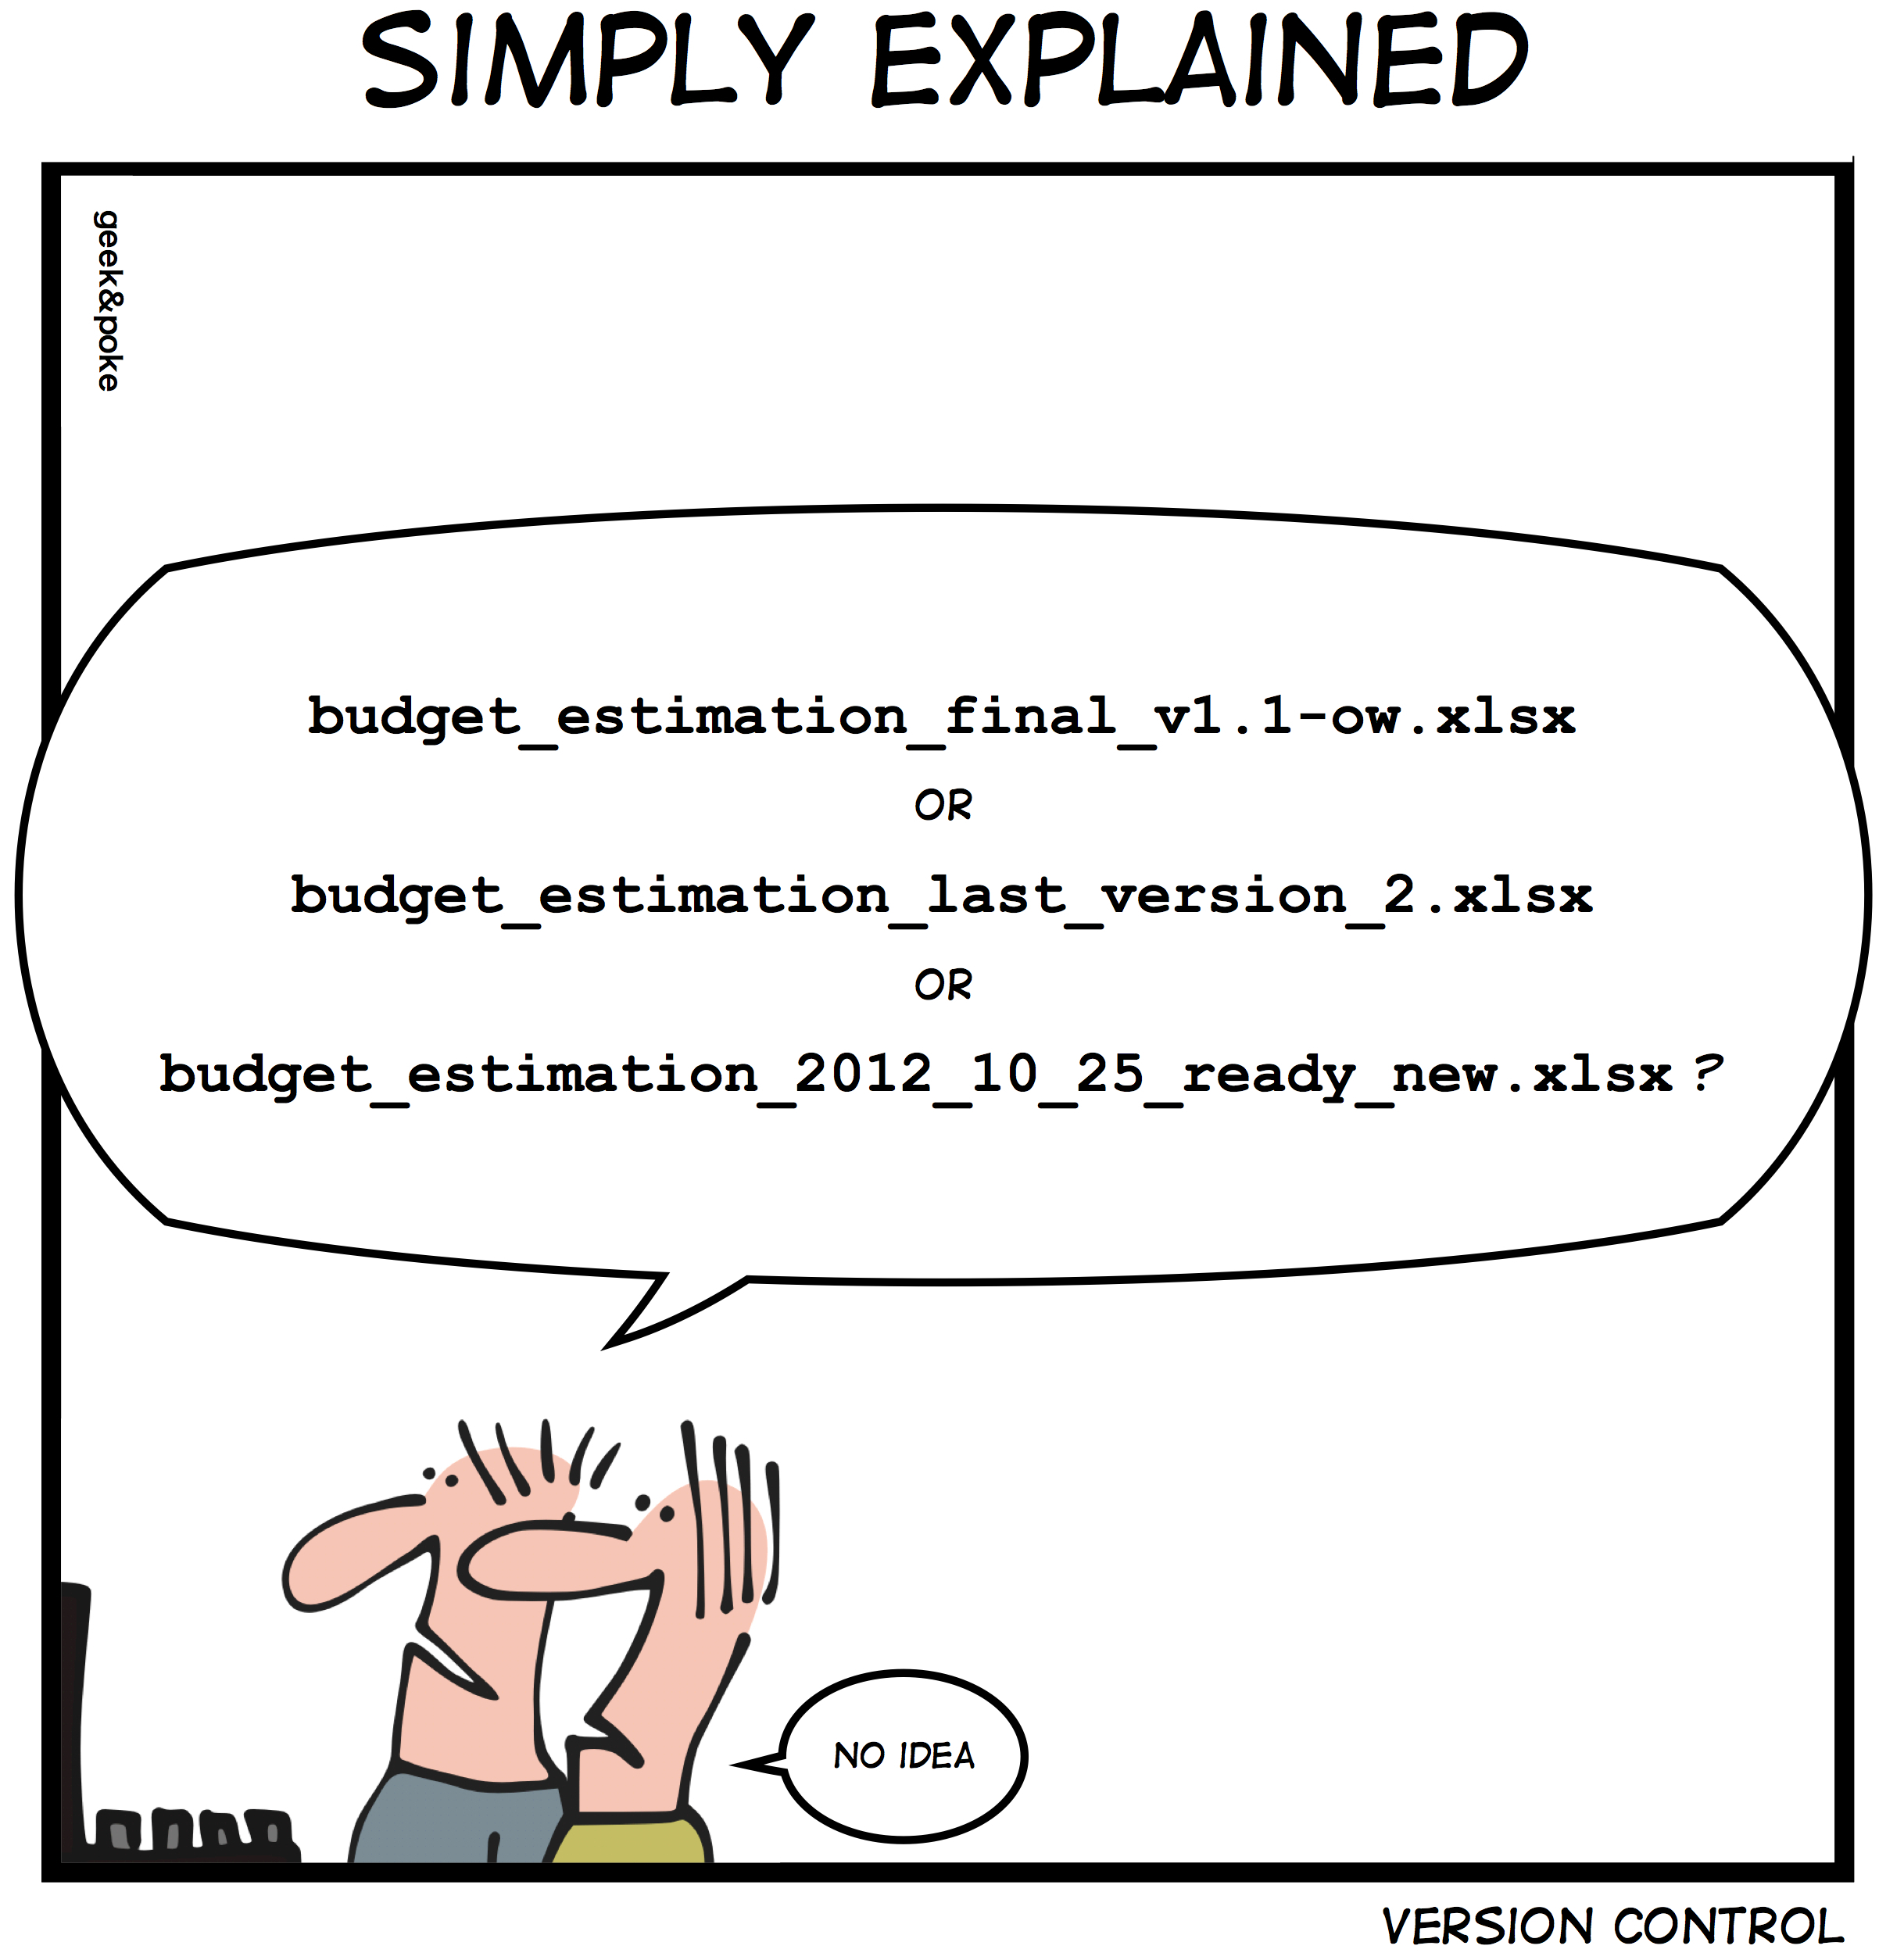
\includegraphics[height=.75\textheight]{why_version_control.jpg}
\end{center}
\end{frame}

\begin{frame}{Motivation}
\begin{itemize}
  \item Implementation of long term change history 
  \begin{itemize}
  \item No ridiculous file names
  \item No archive subfolder
  \item Always perfect overview of file history and changes
  \end{itemize}
  \item Collaborations
  \begin{itemize}
  \item What has changed?
  \item Who has changed it?
  \item Documentation of changes
  \item Parallel working possible (merging)
  \end{itemize}
\end{itemize}
\end{frame}

\begin{frame}{But...}
\begin{center}
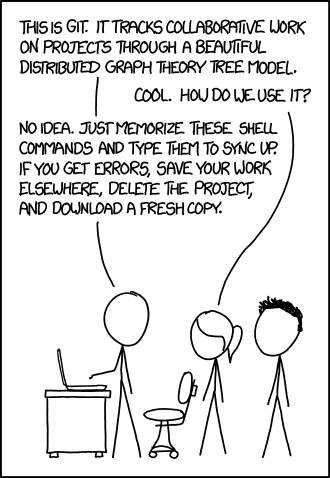
\includegraphics[height=.75\textheight]{git_no_idea.png}
\end{center}
\end{frame}

\begin{frame}{Requirements}
\begin{itemize}
  \item Install git 
  \item Install User Interface for git (RStudio, Gitkraken, ...)
  \item Setup account for Github/Bitbucket/Gitlab/...
  \item Connect everything
\end{itemize}
\end{frame}

\begin{frame}{Workflow}
\textbf{Creating a repository}
\begin{itemize}
  \item Create an online repository (e.g. on Github)
  \begin{itemize}
    \item Use an R specific .gitignore
    \item Initialize with a short readme
  \end{itemize}
  \item Clone the repository to your local machine
  \item (optional) Place an R project in the existing repository
\end{itemize}
\end{frame}

\begin{frame}{Workflow}
\textbf{Working with a repository}
\begin{itemize}
  \item Before working: Synch your local repo (\textbf{Pull})
  \item Perform changes in your local repository
  \item \textbf{Stage} your changes
  \item \textbf{Commit} your changes (aka new version)
  \item \textbf{Push} your changes
\end{itemize}
\end{frame}

\begin{frame}{Recommendations}
\begin{itemize}
  \item Keep it simple! 
  \begin{itemize}
    \item No branches/forks/pull requests
  \end{itemize}
  \item Have meaningful commits
  \item Keep it lean (no big files)
\end{itemize}
\end{frame}

\begin{frame}{Resources}
Git (+ R) Resources
\begin{itemize}
\item Small Intro (\url{https://r-bio.github.io/intro-git-rstudio/})
\item Happy Git with R (\url{https://happygitwithr.com/})
\item R Packages and Git (\url{https://r-pkgs.org/git.html})
\item Git Book (\url{http://git-scm.com/book/en/v2})
\end{itemize}

\end{frame}

\begin{frame}{Literature Recommendations}
R Resources
\begin{itemize}
\item Avanced R Ed. 1 (\url{http://adv-r.had.co.nz/})
\item Avanced R Ed. 2 (\url{https://adv-r.hadley.nz/})
\item R Inferno (\url{https://www.burns-stat.com/pages/Tutor/R_inferno.pdf})
\item R Packages (\url{https://r-pkgs.org/})
\item Clean Code (\url{https://enos.itcollege.ee/~jpoial/oop/naited/Clean\%20Code.pdf)})
\end{itemize}

\end{frame}

\begin{frame}[plain]

\begin{center}
\Large Thank you for your attention!

\visible<2>{Questions? Remarks?}
\end{center}

\end{frame}

\end{document}
